\chapter{Forward converter}
The study model includes, in addition to the transistor control circuit, the following setup:

\begin{figure}[h]
\centering
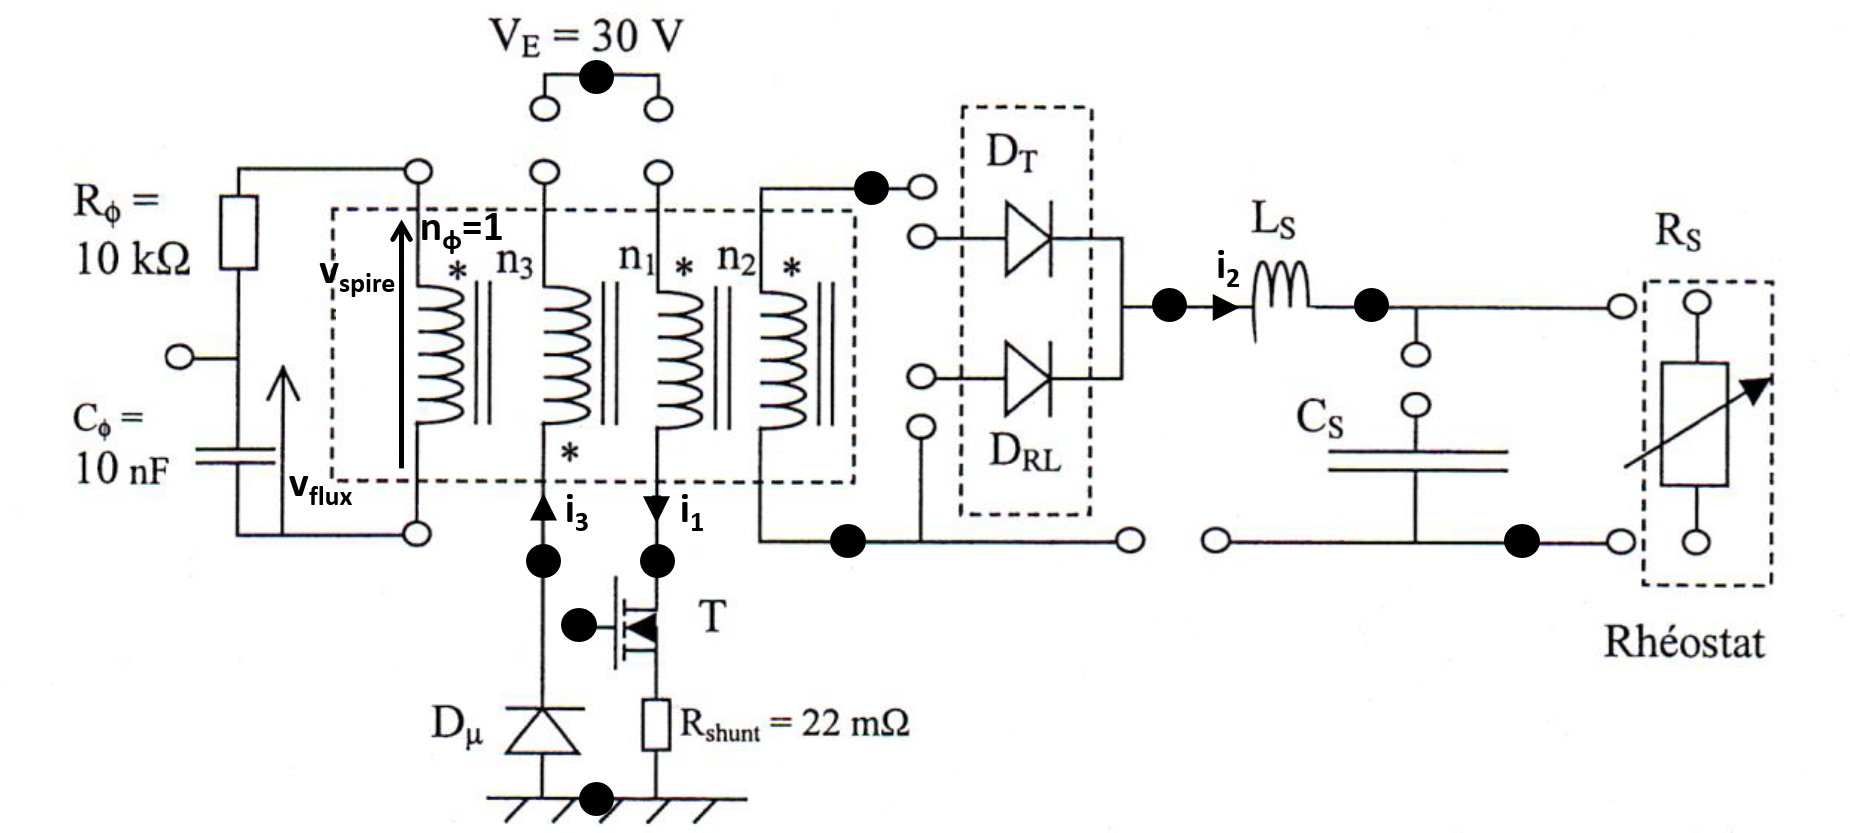
\includegraphics[width=\linewidth]{TP_Forward/fig/Schema_Forward.png}
%\caption{Simplified internal control}
\end{figure}

Test points $\bullet$ allow visualization of various signals, particularly the MOSFET transistor control signal.

The 4 windings are on the same ETD29/16/10 magnetic core made with N27 type ferrite, whose documentation is attached. This core can be equipped with an adjustable air gap using non-magnetic shims. In this case, the relationship between the thickness $s$ of the air gap and the value $A_L$ of the specific inductance is given by the following relation where $K_1$ and $K_2$ are two constants provided in the documentation:
$$s=(\dfrac{A_L}{K_1})^{\dfrac{1}{K_2}}$$

The missing connections should be made using "jumpers" to visualize the currents using appropriate probes. Care should be taken to \underline{\textbf{never disconnect the demagnetization winding}}. The load rheostat can be either 250 $\Omega$ or 330 $\Omega$ indifferently.

Note the presence of a flux measurement circuit made with a single turn connected to an R-C integrator circuit. The voltage $v_{flux}$ thus allows visualization of the flux ripple in the magnetic circuit.

The transistor control device is identical to that of the Flyback power supply (see TP "Flyback Power Supply").

\newpage
\section{Preparation}

Assume the transistor is controlled by a PWM signal with a duty cycle $\alpha=0.25$. Also assume that the converter operates in \textbf{total demagnetization mode} for the transformer and that no load is connected to the converter output. The input voltage $V_E$ is assumed to be constant. The study will focus only on the \underline{steady state}.

\begin{enumerate}
\item Complete the timing diagrams below by plotting:
\begin{itemize}
\item the flux $\varphi$ in the transformer
\item the current $i_1$ supplied by the power supply
\item the current $i_3$ in the demagnetization winding
\item the voltage $v_2$ at the transformer output
\end{itemize}

\begin{figure}[h]
\centering

\includegraphics[width=0.7\linewidth]{TP_Forward/fig/prepa.png}
%\caption{Simplified internal control}
\end{figure}

\item Assume the time constant of the $R_\phi-C_\phi$ filter is much larger than the switching period of the chopper. Show that $v_{flux}$ allows visualization of the flux ripple in the transformer. Determine the flux ripple $\Delta \varphi$ as a function of $\alpha$, $T$, and the value of $v_{spire}$ over the interval $0<t<\alpha T$.
\end{enumerate}

\newpage
Throughout the TP, the following precautions must be taken:

\begin{itemize}
\item use two independent sources to achieve $V_{alim}$ and the "power" supply $V_E$: \textbf{carefully set the current limit of the latter to 2 A}
\item keep the $V_{alim}$ voltage present throughout the session but lower the $V_E$ voltage at each connection modification
\item do not lower the switching frequency below 15 kHz
\item when multiple voltage measurements are made simultaneously with a voltage probe, \textbf{be careful not to create a short circuit}. Indeed, the voltage probes are not isolated from each other, so the potential references of the probes are linked via the oscilloscope
\item \underline{\textbf{never disconnect the demagnetization winding}}
\end{itemize}

\section{No-load operation}

In this first part of the study, there is no load at the power supply output.

\begin{enumerate}
\item Set the switching frequency to 50 kHz and the duty cycle to its maximum value (which will be noted). Observe the voltage across the flux measurement turn $v_{spire}$ as well as the voltage $v_{flux}$. Deduce the peak-to-peak excursion $\Delta B$ of the magnetic induction in the circuit using the documentation ($\Delta B = B_{max} – B_{min}$).

\item Verify complete demagnetization at each period by simultaneously observing the currents $i_1$ and $i_3$. Compare these observations with those of the voltage $v_{flux}$.

\item By simultaneously observing the current $i_1$ and the voltage $v_1$, determine the value of the primary magnetizing inductance, noted $L_1$. What is the value of the used air gap?

\item By comparing the voltages $v_{spire}$ and $v_1$, then $v_2$ and $v_3$ (the voltages $v_i$ are measured across the windings of $n_i$ turns), determine the number of turns $n_1$, $n_2$, and $n_3$. Is this result consistent with the value of $L_1$ found (use the magnetic core documentation)?

\item By simultaneously observing the current $i_1$ and the voltage $v_{flux}$, gradually decrease the switching frequency to 20 kHz while maintaining the maximum duty cycle. What happens?
\end{enumerate}

\newpage
\section{Loaded operation}

Connect the load rheostat after setting it to a value of $30\Omega$ to perform the following measurements. Do not forget to connect all the "open" connections allowing the measurement of the various secondary currents. Set the switching frequency back to 50 kHz and the duty cycle to its maximum value.

\begin{enumerate}
\item Simultaneously and successively observe the following pairs of quantities:
\begin{itemize}
\item the secondary voltage $v_2$ and the voltage across $D_{RL}$, $v_{DRL}$
\item the output current $i_S$ and the voltage across $D_{RL}$
\item the currents in the two secondary diodes, $i_{DRL}$ and $i_{DT}$
\end{itemize}

What can be said about the operating mode of these secondary diodes?

\item Simultaneously observe the current $i_{LS}$ in the inductor $L_S$ and the voltage $v_{DRL}$. Deduce the value of this output inductance $L_S$. What can be said about its sizing?

\item Simultaneously observe the current in the filtering capacitor $i_{CS}$ and the output voltage $v_S$. Deduce the value of the filtering capacitor $C_S$.
\end{enumerate}

\section{Static curves}

The purpose of these measurements is to plot the network of static characteristics at the power supply output. The switching frequency is kept constant at 50 kHz.

\begin{enumerate}
\item For several values of the duty cycle (e.g., $\alpha_{max}$, 0.3, 0.2, 0.1), modify the load rheostat resistance to vary the average current supplied between its minimum value (obtained with the rheostat at maximum) and a maximum value of 2 A. Then record the average values of the current supplied by the power supply $V_E$, $I_E$, the output current $I_S$, and the output voltage $V_S$.

\item Deduce the plot of the characteristics $V_S(I_S)$ parameterized by $\alpha$. Also plot the power transfer characteristics $P_S(P_E)$ and deduce the efficiency.
\end{enumerate}